\chapter{RPGLite: A Mobile Game for Collecting Data}\label{chap:rpglite}

\revnote{About what, and why? Consider changing title. add a sentence in first
  paragraph describing why this fits in with the rest of the dissertation, and
  why it is here.} RPGLite is a game designed to mimic existing popular games,
while being structured to permit exploring all game states via formal
methods;\revnote{Suggest new sentence}
\citeauthor{kavanagh2020}~have produced PRISM models\revnote{PRISM undefined} which can be model-checked
to identify optimal play strategies in all game
states~\cite{kavanagh2020}\revnote{``game states'' not welld efined here, though
I do define it later on}. Some
  experiments were conducted around RPGLite by \citet{kavanagh2021thesis} to
  investigate whether players' interactions with the game converged on optimal
  play.
  \revnote{Lift screenshots in this chapter from game-on paper source where possible}

Real-world play of the game invites many research questions. For example, an
alternative question to answer would be, ``what strategy of play do players
typically adopt?'' or, relatedly, ``do all players adopt the same strategies?''
\footnote{These are not of research interest for the purposes of this thesis,
but examples of interesting questions to ask of a game where ``correct'' and
``incorrect'' actions can be categorised.} \citeauthor{kavanagh2020}'s work can
identify the \emph{``cost''} of an action~\cite{kavanagh2020,kavanagh2021thesis}
as the degree to which a player is less likely to win having made a given move
instead of the optimal one, allowing for richer datasets to be produced and more
in-depth analysis of real-world play to be conducted. One possibility invited by
these datasets is that it may permit modelling of real-world players'
interactions with the game, and therefore offers an opportunity to investigate
the effectiveness of aspect-oriented simulation and modelling.\revnote{From
Jess: this seems important, but needs clarification and reworking. She suggests
moving it to the top.} Referring back to \inline{TODO INSERT RESEARCH QUESTION
HERE}, it would be feasible to build a model of RPGLite play which did not
satisfactorily model real-world data, inviting aspectual augmentation of the
model in an attempt to improve its performance, and thereby investigating the
research question proposed.\revnote{From Jess: The last half of this para in
particular is hard to understand.}

However, it would not be possible to perform analyses of player behaviour
without real-world player data. Datasets collected empirically would be required
to compare against synthetically generated datasets, to ascertain their
similarity and thereby compare different methods of producing synthetic
datasets. As RPGLite is a real-world sociotechnical system which already yields
a formal analysis of play, and datasets from this system can be used to support
multiple avenues of research in different disciplines,\footnote{Later
contributions in this thesis are supported by datasets produced by RPGLite, as
were the contributions of \citeauthor{kavanagh2021thesis}'s PhD
thesis~\cite{kavanagh2021thesis}.} producing a dataset of real-world RPGLite
could also support future work in a variety of fields as a non-commercial
dataset for research in fields including at least game design and gameplay
research~\cite{kavanagh2021thesis}, formal methods~\cite{kavanagh2020},
sociotechnical simulation research, and research software engineering tooling
demonstration.

To that end, a collaboration was undertaken\revnote{J: rework passive voice}
with \citeauthor{kavanagh2021thesis} to develop and release a mobile
implementation of RPGLite which would collect player data for research purposes.
The dataset produced would enable \citeauthor{kavanagh2021thesis} to demonstrate
the utility of their model checking in an empirical
scenario~\cite{kavanagh2021thesis}, and for the purposes of this thesis, it
would also enable the analysis of models representing player behaviour, by
supporting the comparison of these models against the collected data.

\revnote{J: this para's easier to understand than previous ones in this chapter.
  When reworking, consider how the others could be rewritten in a style closer
  to this? She also notes it might belong further up in the chap.}The
development and release of RPGLite as a mobile game offers an opportunity to
make use of aspect orientation in a new context: a model of naive RPGLite play
can be produced\revnote{J: avoid passive voice} which represents random play,
and aspects could be written which augment the naive model representing
hypothesised player behaviour. If the aspectually augmented models generate data
which correlates with empirically sourced data more closely than that generated
by the naive model (with random play, and no aspectual augmentation), we can
dismiss naive play as ``realistic'', and understand the aspectually augmented
behaviour as ``more realistic''. Many aspects can be written representing
different styles of play, which might be adopted by different players, a
concrete benefit of aspect orientation in modelling \& simulation.

\revnote{J: She suggests moving this earlier, too.}The modelling \& simulation
research opportunities RPGLite presents are realised in
\cref{chap:exp1_simulation_optimisation} and
\cref{chap:exp2_old_aspects_new_systems}; this chapter focuses only on the
design and development of RPGLite as a mobile game, and the dataset collected
from real-world play and released
~\cite{RPGLiteLessonsLearned}. It starts with an overview of
RPGLite itself in \cref{sec:rpglite_overview}, and progresses to a discussion of
the game's implementation in \cref{sec:rpglite_implementation} before concluding
with a discussion around the empirical data collected using the game in
\cref{sec:rpglite_data_discussed}.

\section{An Overview of RPGLite}\label{sec:rpglite_overview}\revnote{Needs copy-editing}

RPGLite is a simple two-player game played in turns. Each player selects
characters independent of the other, with each character having a unique set of
abilities and properties, which are generally health, chance of success on
attack, and damage dealt on a successful attack. The abilities of some
characters necessitate additional properties. Each player selects an ``alive''
character (one with health greater than 0) to perform their action against a
chosen ``alive'' target (or occasionally targets). A successful attack ---
randomly determined by chance of successful attack for the selected attacking
character --- results in that character's unique ability being inflicted on
their target[s]. A random player is chosen to take a first move, players may
always skip their turn as a valid action, and players continue to take
alternating turns until a victor is left with the only ``alive'' characters.

Eight characters are available for selection, with the following
abilities\revnote{J: compress the description list. Maybe make it bulleted? I
  wonder whether it can just be a para or something.}:

\begin{description} \item[Knight] Deals damage to an opponent character on a
successful hit.  \item[Archer] Deals damage to two opponent characters on a
successful hit.  \item[Wizard] Deals damage to an opponent character on a
successful hit, disabling (or \emph{``stunning''}) them for the duration of the
opponent's next turn.  \item[Healer] Deals damage to an opponent character on a
successful hit, and heals themselves or, optionally, the other player character
instead (assuming that character is still alive).  \item[Barbarian] Deals damage
to an opponent character on a successful hit, dealing additional damage if
their\revnote{J: whose? the barbarian's? Clarify.}
health is low when attacking.  \item[Rogue] Deals damage to an opponent
character on a successful hit, dealing additional damage if the target's health
is low when attacked.  \item[Monk] Deals damage to an opponent character on a
successful hit, and immediately takes another turn, until their attack is
unsuccessful.  \item[Gunner] Deals damage to an opponent regardless of success,
dealing additional damage on a successful hit.  \end{description}

Specific details of each character --- their health, chance to hit, and damage
on hit as well as character-specific details (such as the threshold for
additional Barbarian or Rogue damage, for instance) --- are defined as a
\emph{``configuration''} of RPGLite. Different configurations change the game's
\emph{``balance''}, a term referring to the relative strengths of different
characters or character pairs. For example, if a configuration leaves many
characters with initial health values close to a Barbarian's threshold for
additional damage, then they become a very powerful character due to their
ability to inflict additional damage. If the Monk's chance to hit is high, the
repeated turns it offers can be very advantageous. Character skills can work in
concert with each other: choosing a Barbarian and Healer such that the barbarian
can be kept at low health for additional damage, but the healer can be used to
keep them alive, may be an effective strategy depending on the game's
configuration. \citeauthor{kavanagh2019balancing} found that model-checking a
configuration of the game could discover the relative strengths of characters
and character pairs when played optimally~\cite{kavanagh2019balancing}.

RPGLite's design has two objectives it must meet. First, that it is interesting
to players, which requires that it is approachable and complex enough not to be
immediately solvable. This is necessary for real-world data collection, and to
demonstrate a design representative of something that could conceivably be a
real-world game with an active playerbase. Second, RPGLite's design must be
sufficiently simple for model-checking. Model checking is a necessary
requirement of design because of our need to identify optimal moves: analysis of
player behaviour rests on our understanding of how close to ``ideal'' players
are, and whether players approach ideal strategies over time. This is the crux
of the work found in formal methods research on
RPGLite~\cite{kavanagh2021thesis,kavanagh2020}, which relies on a reduced state
space in order to calculate optimal moves and character pairings.

\subsection{RPGLite's Design Implications}

The state space\revnote{Jess noted this wasn't formally described. I describe it
later, but clearly it's confusing on a first read; consider either reordering or
including a definition earlier, the term shouldn't be used here if it's not
defined properly.} of RPGLite makes it unusually well-suited to analysis through
formal methods.  Because of this, datasets produced through simulation of
RPGLite can be compared against two other datasets: one of real-world play, and
another of what can be mathematically shown to be ``correct'' player behaviour.

To demonstrate this state space, note that RPGLite games can have their states
described\revnote{J: so is that the state, or just a description of a subset?
  (It's a complete and uniquely identifying state, but I don't make this clear enough)} by a set of values: the healths of characters on each team, plus a
stunned character. With eight characters each having their own maximum health
value, which we denote $w, x,
y, z$\footnote{Maximum health values are dependent on RPGLite's configuration.},
two players, and an indicator of which character is stunned.\footnote{Note that
stunnedness is valid for exactly one character for one turn, meaning that only
one character may be stunned at any time, and the status effect immediately
resets, meaning there are only three possible states for stunnedness: either
character belonging to the player taking a turn, or neither.}. The
entropy\revnote{J: define earlier? Also: why is entropy important here?} of a
game's state is therefore
\(log_2(w\times{}x\times{}y\times{}z\times{}3\times{}2)\)\revnote{J: does the
  order matter?}, where the
multiplications by 3 and 2 represent the stunnedness indicator for the current
player (either character, or neither), and the player whose turn it is to play,
respectively. The maximum health for a character is 10 hit points, which makes
the maximum entropy of a game state \(log_2(10^{4}\times{}3\times{}2\}) =
log_2(60000) \approx 16.87 bits\). Each player picks 2 of 10 characters, and can
choose to attack either opponent character with either of their own, or skip
their turn, for a maximum of 6 possible actions. We can therefore see that the
total entropy of the entire RPGLite game is no greater than
\(log_2(10^{4}\times{}6\times{}2\times{}{10\choose2}\times{}6 \approx 24.36
bits\)\revnote{J: Summarising her notes but 1. Footnote should be integrated
  into body and 2. Entropy's a confusing concept, wasn't
  what she was expecting here for defining a state space. Either make the
  concept extremely clear or, better, avoid the concept of entropy so as not to
trip people up. Clearer writing > clever writing.}.\footnote{
  The actual figure is smaller: 
  \begin{itemize}
    \item Players may choose two characters with special abilities that prevent
    them from attacking both opponent characters at once (this accounts for 9
    out of 10 characters), giving 5 possible actions in a turn rather than 6.
    \item Players are likely to judge different strategies to be more effective
    at different times due to their assessment of others' strategies: certain
    decisions might be poor in general but successful in certain circumstances.
    If a player determines that a certain strategy is ``popular'', they may
    assume their opponent will play in the popular manner and adapt their own
    strategies
    accordingly~\cite{howard1971metagames_seminal,metagaming_in_esports}.
    RPGLite is designed to have slightly ``unbalanced'' parameters of different
    characters such as health, attack damage, or potency of special abilities,
    meaning long-term players are expected to learn effective playstyles and
    adjust accordingly.
\end{itemize}\par{}\indent{}
Players' behaviour
is therefore less uniform than this calculation would imply, but the calculation
provides a higher bound on the entropy of the game.
}

Iterating through these states allows us to map the entire state space of
RPGLite. As the state space the game defines is relatively small\footnote{For
comparison, mapping valid positions in chess takes about 136
bits~\cite{information_content_chess}, and this figure does not account for
valid \emph{moves} within the game, which our calculation for RPGLite does} 
it is feasible to analyse every possible game state. Note that the figure of
\(\approx 24.36 bits\) includes movements \emph{between} states as well as the
states themselves, meaning that it is feasible to map the potential progressions
through all possible games of RPGLite using formal methods. Further, this allows
us to understand the chances of a player winning given transitions between
different states, for example by representing moves in the game as transitions
in a decision diagram\revnote{J: suggest a diagram here} where nodes are the game's state. We can calculate exactly
how ``good'' a move is, by comparing chances of success\revnote{J: this needs to
be defined too} when making a given move in a
given state against the chances of success when making the objectively optimal
move.

In this way, RPGLite's design allows it to be understood formally, yet it also
draws on common game design elements and is sufficiently ``interesting'' to
generate data from a real-world playerbase.\footnote{Demonstrated through data
collected from several thousand completed games, which can be found at
\cite{rpglite_dataset}.} This yields some useful properties for the purposes of
aspect-oriented simulation\revnote{J: first section isn't clear, she notes she
  didn't understand. In second section she circles ``known'', asking, ``known by
  whom?''}:

\begin{enumerate} \item Simulated moves can be selected naively, i.e. at random,
but can also be made perfectly according to the known-correct move in a given
game state, or made with some calculated ``cost'' as to the chance of winning.
\item Real-world players' behaviour can also be analysed according to the same
metrics: for example, moves made by players can be analysed to understand bias,
whether players learned to play ``better'' moves over time, or whether they
selected known-strong characters more frequently than those who can be formally
shown to have a relatively low chance of winning games.  \item As the actions
taken when playing RPGLite are consistent --- such as deciding the target
character of an attack, or a character to use in an attack --- random play can
be simulated as a ``naive'' play style, which can be compared against real-world
players. Where player behaviour does not correlate to naive
play,\revnote{Footnote suggests correlation is defined in chap 6; include a more
specific cref.}\footnote{The
concept of play correlation is introduced in
\cref{chap:exp1_simulation_optimisation}.} the biases of players may be
represented as aspects which are applied only to specific actors within the
simulation.  \item Should aspects be suitable as a manner of accurately
representing biased play, aspects offer a separation of concerns within the
simulation: any nuance found within the playstyle of specific real-world players
would be replicated and applied not to the model itself, but to specific
simulated players. Playstyles might also be mixed with the application of
multiple aspects.  \end{enumerate}

Whether aspect orientation is suitable for the realistic simulation of RPGLite
gameplay is the topic of the remainder of this thesis. However, the design of
RPGLite allows for a controlled system where a clear notion of ``good'' and
``naive'' behaviours can be defined, the system is closed insofar as all
interactions within the system are known and all game elements are precicely
understood, and all interactions take place between experiment participants for
data collection purposes, allowing for a large dataset to be collected without
information being removed due to players not consenting to their data being
collected and disseminated for science. In short, RPGLite's design constitutes a
system where all aspects are well-understood, no interference is anticipated
from system components which are unknown or outside of experimental control, and
lots of data can be collected for analysis. Therefore, the data generated by
gameplay is suitable for comparison against datasets outputted through
aspect-oriented simulation. This can be used to assess whether simulated players
with aspect-affected behaviour accurately reflect the playerbase, and so can
help to assess whether aspect orientation is suitable for realistic simulation.

% can be represented as modifications to naive play modificationsReal-world
% player data can be compared against simulation data with biases repre to
% identify 

\section{Implementation of RPGLite}\label{sec:rpglite_implementation}

\revnote{J: compress}Knowing ideal play is useful. However, to understand how real-world players
would interact with RPGLite, empirical data needed to be collected. To produce
this, a mobile online multiplayer version of the game was developed for data
collection purposes. Play constituted engagement with an experiment for data
collection, and after several months, a database logging player behaviour
offered a dataset which could be used to simulate real-world player behaviour.
%  and present a ``realistic'' environment in which to test the effectiveness of
%  aspect-oriented simulation.

This section describes details of RPGLite's implementation as a data collection
tool. Some lessons learned after reflection on the implementation process were
documented for the benefit of others' avoiding our
errors\cite{RPGLiteLessonsLearned}\revnote{Should a summary of the paper be a section
here, or maybe an appendix? Keen not to plagarise, but it's also maybe worth
including. William and I both spent a lot of time getting that paper out. I
presented it at GameOn2020. He's included some in his thesis, so I guess it's a
precedent for me to do the same. And why not?}.

\subsection{Consent to participation}\label{subsec:consent_to_participation}

% \inline{Include notes \& screenshots here explaining that users were prompted
% in-app to accept their data being recorded and published for research
% purposes, and that the data collected was used \emph{only} for research
% purposes, that no personally identifying data was collected, and that data
% collection was signed off by the University of Glasgow ethics committee. Users
% could not create an account without accepting that their play data would be
% collected and published for research purposes, and users could withdraw that
% consent at any time. Further information was also made available at
% \url{rpglite.app}}

Players gave consent to participate in a scientific study as a part of creating
an account to play RPGLite. Players were required to explicitly scroll through
an information sheet and consent agreement and agree to both to make an account.
Copies of both were made available to download for player reference in both the
game and RPGLite's website\footnote{RPGLite's website is available at
\href{https://rpglite.app/}{https://rpglite.app/}, where copies of the consent
form and information sheet are linked.}\revnote{Should info sheet / consent form
be cited, instead of linked as in this footnote\ldots{}?}. Players were instructed to
contact the involved researchers to withdraw participation, and were instructed
that they could do so at any time. Email addresses to contact were noted in both
the app and the website.

The study, information sheet, consent form, and data collected were reviewed by
the University of Glasgow Science \& Engineering ethics committee before the
game was publicly released.

\subsection{Mobile app}

As a mobile game, RPGLite's user-facing component was an application,
distributed through the Google Play Store on Android and the Apple App Store on
iOS. This was developed in Unity, a framework for developing games in C\# which
can be distributed to almost any platform. Most assets were developed in GIMP, with character designs
contributed by a commissioned artist online. Unity allowed for a ``WYSIWYG'' or
what-you-see-is-what-you-get interface builder, with event handlers defined in
C\# code which would ``hook'' into events signalled by interface element
interactions. \revnote{J: rest of this para should be made shorter.}User-facing components of the game were largely produced by
\citeauthor{kavanagh2021thesis}, the collaborator on this project and original
RPGLite designer. Therefore, in an attempt not to take credit for this component
of the work involved in collecting the RPGLite dataset, curious readers are
referred to \citeauthor{kavanagh2021thesis}'s notes on the development process
for full details~\cite{kavanagh2021thesis}.

Beta testing required user engagement. Apps were deployed to Android and iOS
devices of colleagues, who played a series of games to check that game logic was
sufficiently robust and graphic design sufficiently adequate for public
distribution of the game. In a manner inspired by design science
methodology~\cite{johannesson2014introduction}, beta tests comprised of
iterations on the artefact of the game and its server-side component (discussed
in \cref{subsec:server-side-logic}) which were distributed to beta testers.
Informal feedback and enhancement requests were sought on each iteration until
the game behaved correctly in all edge cases (no major bugs were reported) and a
final design was settled upon (no major complaints about interaction or
aesthetics were reported), at which point the game satisfied criteria for public
distribution.

An example of the game's visual evolution is given in
\cref{fig:matchmaking_screen_improvements}, where colourful buttons replace a
tabular, text-heavy interface. Another example is the evolution of the game's
main screen, ``Active Games'', which loaded when players logged into the app and
allowed users to see and interact with active games they were involved in. The
visual identity and colour palette of this screen was refined iteratively, as
can be seen in \cref{fig:homescreen_evolution}. Other features which were
developed following user feedback while beta testing include the implementation
of a notification system and a leaderboard showing a player's experience
relative to their peers; these are shown in
\cref{fig:extra_rpglite_features}.\revnote{There are some good screenshots in
the paper for RPGLite; lessons learned. Consider adding those here instead; the
screenshots I've included at present come from my iCloud photos library\ldots{}} 

\begin{figure}
    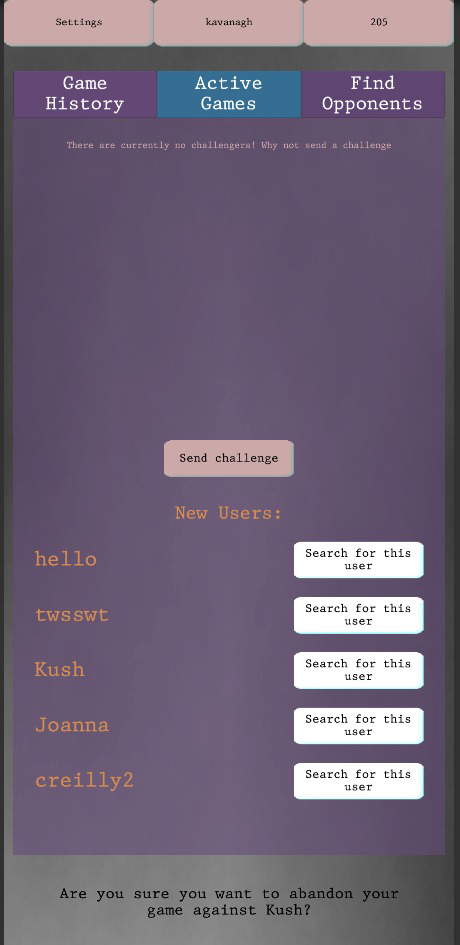
\includegraphics[width=.3\textwidth]{50_rpglite/images/find_users_1.jpeg}\hfill
    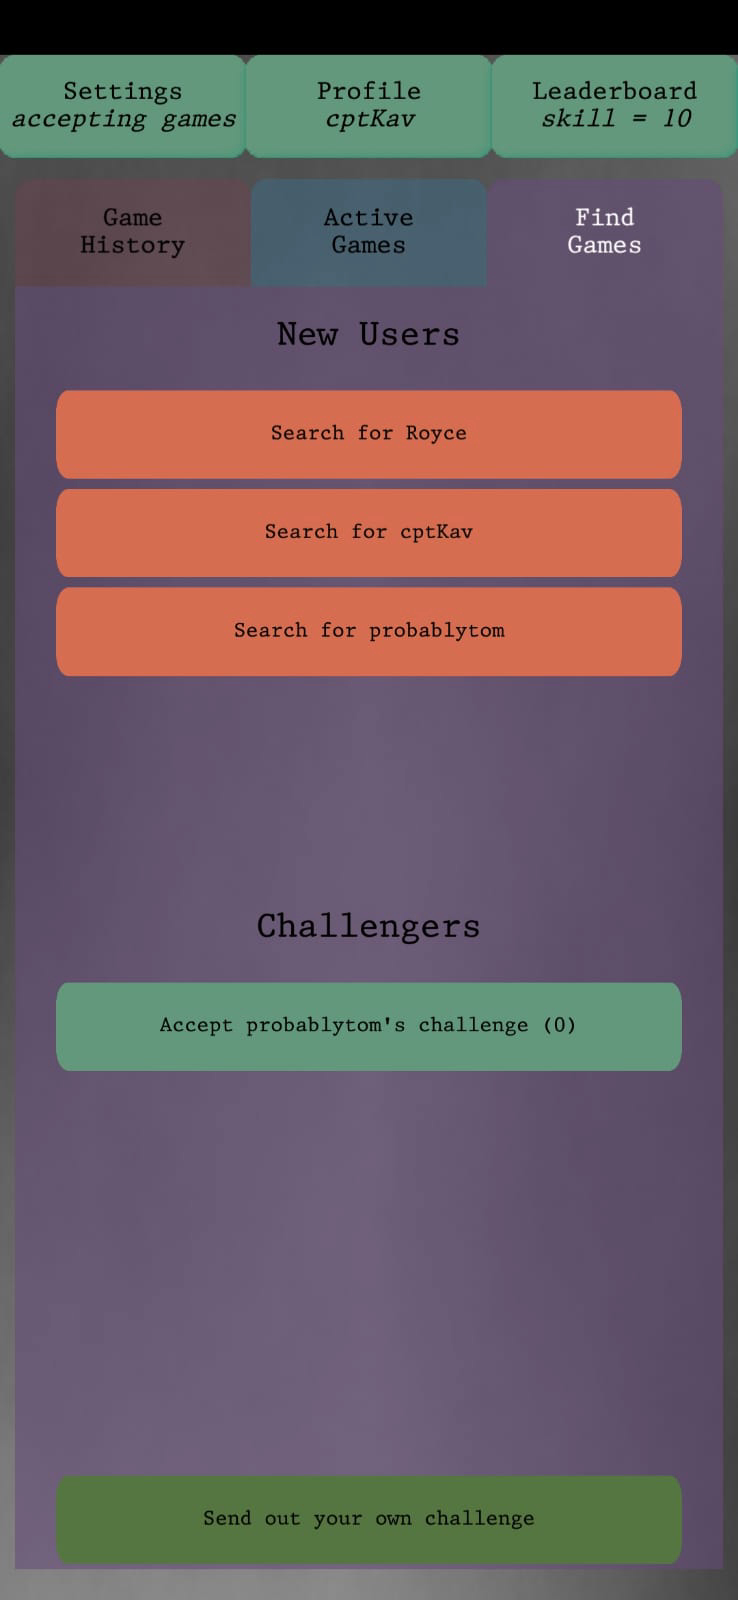
\includegraphics[width=.3\textwidth]{50_rpglite/images/find_users_2.jpeg}
    \caption{Evolution of the ``Find users'' matchmaking screen. Prototype left, final design right.}
    \label{fig:matchmaking_screen_improvements}
\end{figure}

\begin{figure}
    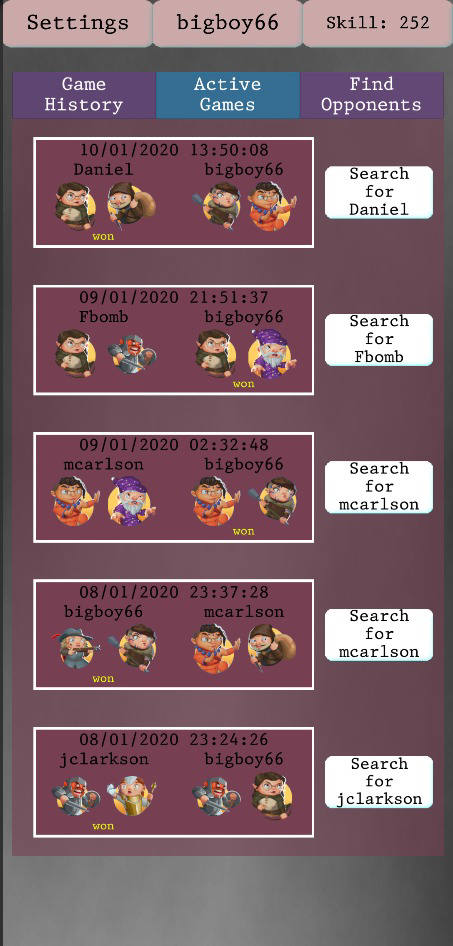
\includegraphics[width=.3\textwidth]{50_rpglite/images/homescreen_1.jpeg}\hfill
    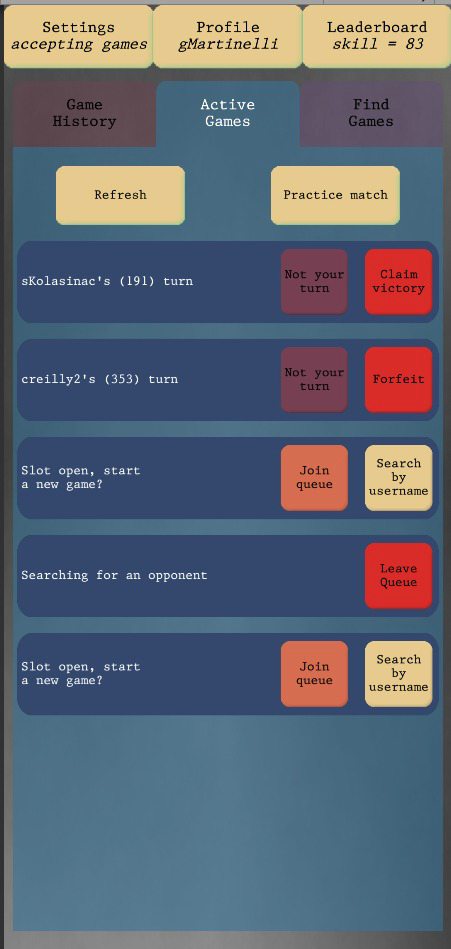
\includegraphics[width=.3\textwidth]{50_rpglite/images/homescreen_2.jpeg}\hfill
    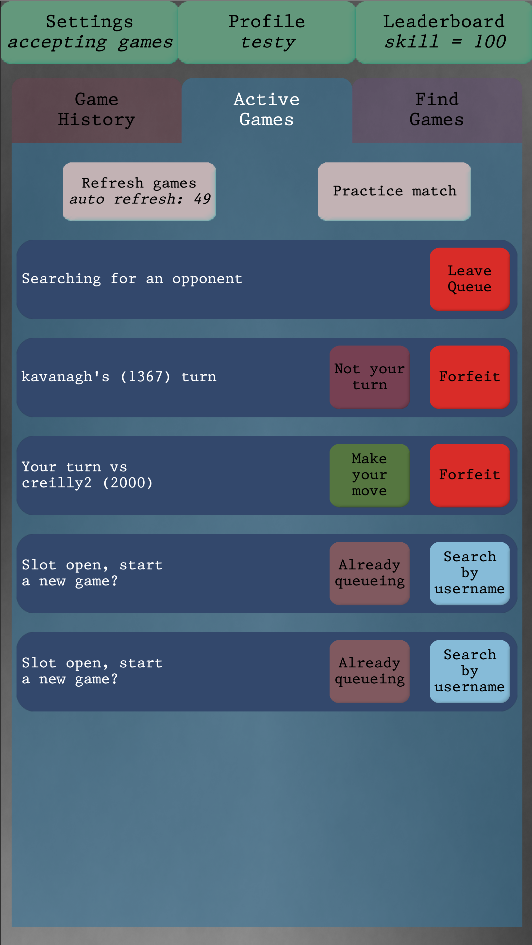
\includegraphics[width=.3\textwidth]{50_rpglite/images/homescreen_3.png}
    \caption{Evolution of the ``Active Games'' screen, which allowed RPGLite users to see and interact with games they were playing. An early prototype is shown to the left; a refinement through beta testing in the center; and the final version released to the public to the right, with an improved colour palette.}
    \label{fig:homescreen_evolution}
\end{figure}

\begin{figure}
    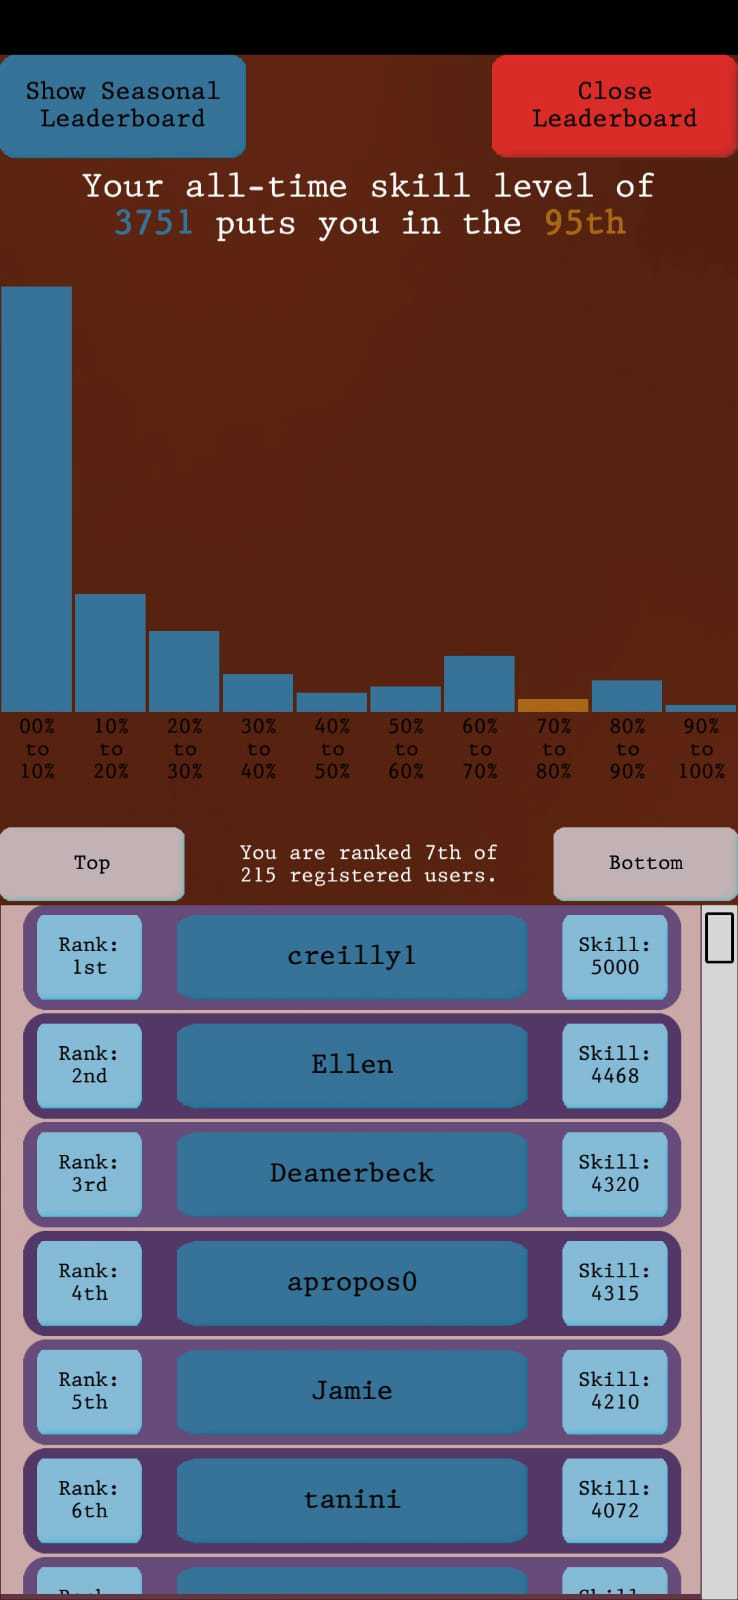
\includegraphics[width=.3\textwidth]{50_rpglite/images/leaderboard.jpeg}\hfill
    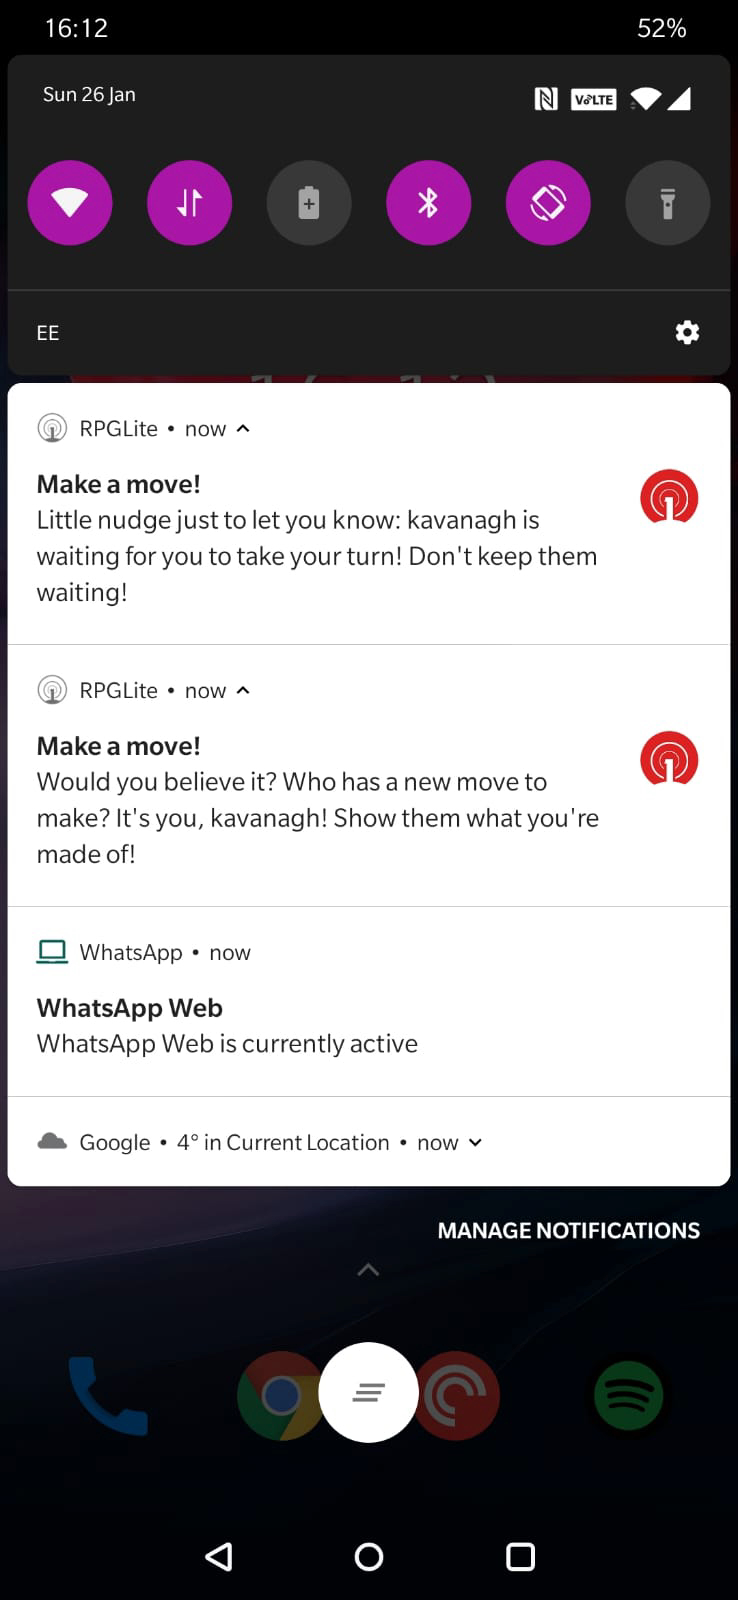
\includegraphics[width=.3\textwidth]{50_rpglite/images/notifications.jpeg}
    \caption{Features developed following requests from beta testers. A leaderboard of player engagement is shown to the left; examples of notifications when an opponent has acted are shown to the right.}
    \label{fig:extra_rpglite_features}
\end{figure}


\subsection{API \& Server-side Logic}\label{subsec:server-side-logic}

As the data collected ought to be empirical\revnote{J: how could the data not be
empirical?}, RPGLite was developed as an online
game. This required a server and API for a client to communicate with.

A REST API was developed with Python's \emph{Flask} framework. Endpoints were
created to support all in-game actions requiring centralised state (or a
recording of that state), allowing for player search, matchmaking, player
profile design, game history and statistics analysis, ranking calculations,
login and password reset, synchronisation of access to sensitive information,
and other in-game activities. The API also allowed moves to be made, and
rejected erroneous game states or unauthorised input from any malicious actor,
to ensure that the data collected, analysed, and published was not manipulated.
The API also sent push notifications to an opponent's device when moves were
made. This was a feature requested during beta testing, which was anecdotally
observed to increase engagement with the game.

On each of these actions, data was collected about the action performed, and
logged in a database. In addition, in-game activities which required no
server-side input but were considered to have potential in later analysis would
log datapoints through the API into the same database.

A MongoDB database instance was installed and managed on a University of Glasgow
Computing Science virtual machine. The no-SQL nature of the database permitted
flexible structuring of the data, and simplified analysis of the games' results
after data collection was completed. The API was also hosted on the same virtual
machine. A combination of port access rules applied via Nginx and hardening the
security of the database itself through MongoDB's account features and
controlled permissions within the server prevented unauthorised access to the
database, ensuring that the data remained untampered.

Game state was interpreted client-side. The intention in this design choice was
to un-burden a centralised service we were responsible for maintaining, moving
functionality such as calculating game states after moves were created to
clients on players' devices. This left the serverside logic mostly concerned
with executing database transactions and ensuring the integrity of game states
was uncompromised. Reflections on the suitability of this approach made after
the game's launch have been published separately~\cite{RPGLiteLessonsLearned}.


\subsection{Data Collected}
\label{sec:rpglite_data_discussed}

In total, players produced a dataset of $9,693$ games. In addition, it includes
$1,105,065$ datapoints generated by gameplay or player interaction with the
client, such as players checking their position on a leaderboard, searching
their game history, or rolling to hit as part of an attack. The data is
drawn\\revnote{J: present here, past elsewhere, be consistent with tenses}
directly from the MongoDB database used to run the game. With player consent on
signup (see \cref{subsec:consent_to_participation}) this data is published and
available for all researchers to analyse in the format of a JSON
object~\cite{rpglite_dataset}.

Completed games drawn from the MongoDB instance contain many fields. The breadth
of datapoints logged by player interaction with the RPGLite app means there are
an extremely broad range of datapoints available to curious
researchers.\revnote{J: make more concise. (I made slight edits when adding this
  revnote, maybe the para can be condensed. I haven't done much right now.)} A full
list of available data is available in a text document within the
dataset~\cite{rpglite_dataset}. Some of particular interest include:

\begin{itemize}
    \item The history of moves made, and the times those moves were
made
\item The players involved and the winning player of each game (by username as
no personally identifying data was collected)
\item The ELO\revnote{ELO undefined.} scores of players in each game
\item The characters chosen by each player
\item The ``score'' of each player\revnote{J: ``score'' is vague. I clarify in
    the footnote but it should be in the body here. Also, ``score'' is not of
    interest. We don't use it in the experiments, don't waste attention on it.}\footnote{RPGLite's mobile app presented users
with a naive scoring mechanism used to rank users on a leaderboard which some
users then used to identify other players of a similar notional skill.}
\end{itemize}



\section{RPGLite Seasons}
\label{seasons_of_rpglite}

RPGLite was played through two ``seasons'': after an initial 3,000 games
played, the game was updated and a second configuration was released. This meant
that, having learned a strategy to play with the initial configuration (such as
a preference of characters) changes were made which may invalidate what players
had learned. The dataset therefore contains two conceptual subsets: data
collected from a system with the same mechanics but tweaked parameters,
resulting in different optimal character pairs and moves. Parameters for
characters in season 1 are given in \cref{fig:s1_config}, in
\cref{fig:s2_config} for season 2, and the differences between the two
configurations are summarised in \cref{fig:changes_between_seasons}.

\begin{figure}[h]
  \begin{minipage}{.50\columnwidth}
    \centering
    \begin{tabular}{@{}l r r r@{}}
      \toprule
      \emph{Character} & \emph{Health} & \emph{Hit Accuracy} & \emph{Damage}\\
      \midrule
      Knight & 10 & 0.60 & 4 \\
      Archer & 8 & 0.85 & 2 \\
      Wizard & 8 & 0.50 & 2 \\
      Rogue & 8 & 0.75 & 3 \\
      Healer & 10 & 0.85 & 2 \\
      Barbarian & 10 & 0.75 & 3 \\
      Monk & 7 & 0.80 & 1 \\
      Gunner & 8 & 0.80 & 4 \\
      \bottomrule
    \end{tabular}
    \caption{Configuration for RPGLite\\in season 1.}
    \label{fig:s1_config}
  \end{minipage}%
  \begin{minipage}{.50\columnwidth}
    \centering
    \begin{tabular}{@{}l r r r@{}}
      \toprule
      \emph{Character} & \emph{Health} & \emph{Hit Accuracy} & \emph{Damage}\\
      \midrule
      Knight & 10 & 0.80 & 3 \\
      Archer & 8 & 0.85 & 2 \\
      Wizard & 8 & 0.50 & 2 \\
      Rogue & 8 & 0.70 & 3 \\
      Healer & 9 & 0.90 & 2 \\
      Barbarian & 9 & 0.70 & 3 \\
      Monk & 7 & 0.75 & 1 \\
      Gunner & 8 & 0.70 & 4 \\
      \bottomrule
    \end{tabular}
    \caption{Configuration for RPGLite\\in season 2.}
    \label{fig:s2_config}
  \end{minipage}
\label{fig:table_of_char_params_between_seasons}
\end{figure}

In the second configuration, most character pairs have their hit accuracy
reduced by 0.05 percentage points. Only the knight's damage is reduced, from 4
points to 3. Health is set to 9 for the Archer, Healer, and Barbarian. This
change alters RPGLite's metagame, as making certain characters weaker and others
stronger incentivises different strategies of play: different character pairs
and moves are optimal as a result of the changed configuration. Player response
to changed configuration is analysed using formal methods by
\citet{kavanagh2021thesis}.

\inline{
  Ideally we'd say a little more about RPGLite's two seasons, but I'm not sure
  exactly what to say. We've got the important details here. Expand if there's
  time; if there's not, that's OK, add more before the viva.
}


\begin{figure}[h]
  \centering
  \begin{tabular}{@{}l l r r@{}@{}}
    \toprule
    \emph{Parameter} & \emph{Character} & \emph{Old Value} & \emph{New Value} \\
    \midrule
    \multirow{7}{*}{Hit Accuracy} & Knight    & 0.60 & 0.80 \\
                                  & Archer    & 0.85 & 0.80 \\
                                  & Rogue     & 0.75 & 0.70 \\
                                  & Healer    & 0.85 & 0.90 \\
                                  & Barbarian & 0.75 & 0.70 \\
                                  & Monk      & 0.80 & 0.75 \\
                                  & Gunner    & 0.75 & 0.70 \\
    \midrule
    \multirow{1}{*}{Damage}       & Knight    & 4    & 3    \\
    \midrule
    \multirow{3}{*}{Health}       & Archer    & 8    & 9    \\
                                  & Healer    & 10   & 9    \\
                                  & Barbarian & 10   & 9    \\
    \bottomrule
  \end{tabular}
  \caption{Altered values of different parameters when moving from season 1 to season 2.}
  \label{fig:changes_between_seasons}
\end{figure}
